\tikzsetnextfilename{ADC-SnH}
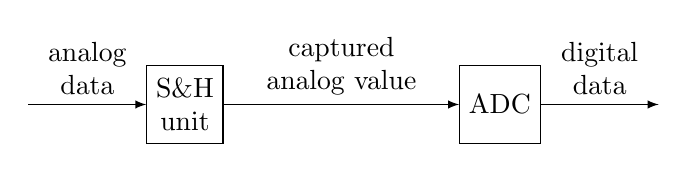
\begin{tikzpicture}[>=latex]
	\node[draw,minimum height=1cm,align=center] (snh) at (0,0) 
    {S\&H\\ unit};
	\node[draw,minimum height=1cm] (adc) at (4,0) {ADC};
  \draw[<-] (snh.west) -- +(-1.5,0)
    node[midway,above,align=center] {analog \\ data};
  \draw[->] (snh.east) -- (adc.west)
    node[midway,above,align=center] {captured \\ analog value};
  \draw[->] (adc.east) -- +(1.5,0)
    node[midway,above,align=center] {digital \\ data};
\end{tikzpicture}